%------------------------------------------------------------------------------
%	CAPITOLO 11
%------------------------------------------------------------------------------

\chapter{Fammi lume}
Il signor \index[Personaggi]{Massaroli Giacomo}Giacomo Massaroli\footnote{\textbf{Giacomo Massaroli}, fu Paolo Antonio, probabilmente parente di quel  \index[Personaggi]{Massaroli Paolo}Paolo Massaroli la cui figlia Aunita\index[Personaggi]{Massaroli Diana Anna Cristina `Aunita'} sposò \index[Personaggi]{Fernè Ferdinando}Fernè Ferdinando} aveva un fido servitore detto ...\footnote{Mingazzi ha omesso il nome}\\
Alla sera quando rincasava, voleva andare nel cortile, con voce baritonale e forte chiamava il buon servitore, il quale era pronto e premuroso.\\
\indent Una sera il signor \index[Personaggi]{Massaroli Giacomo}Giacomo chiamò il servitore perché gli rischiarasse il cammino. Ma il buon servo, accendeva fiammiferi su fiammiferi, diceva sempre <<Vengo, un momento, mi perdoni, ecc>>.\\
\indent Intanto il padrone s'impazientiva\footnote{Si spazientiva} e chiamava più forte. La candela non si accese, e quando il servitore ebbe terminato i fiammiferi, prese la laterna e col padrone entrarono al buio in casa.\\
\indent Finalmente alla luce, di casa, il mistero della mancata accensione si chiarì: uno spirito allegro aveva sostituito alla candela un torso imitazione di radice con entro uno stoppino.\footnote{Qualcuno aveva sostituito la candela con una radice e vi aveva inserito uno stoppino}\\
\indent Per gustare la scenetta bisognava conoscere l'impazienza del padrone e la timida premura del servitore.


\begin{figure}[htb]
    \centering
    %\vspace{-0.7cm}
    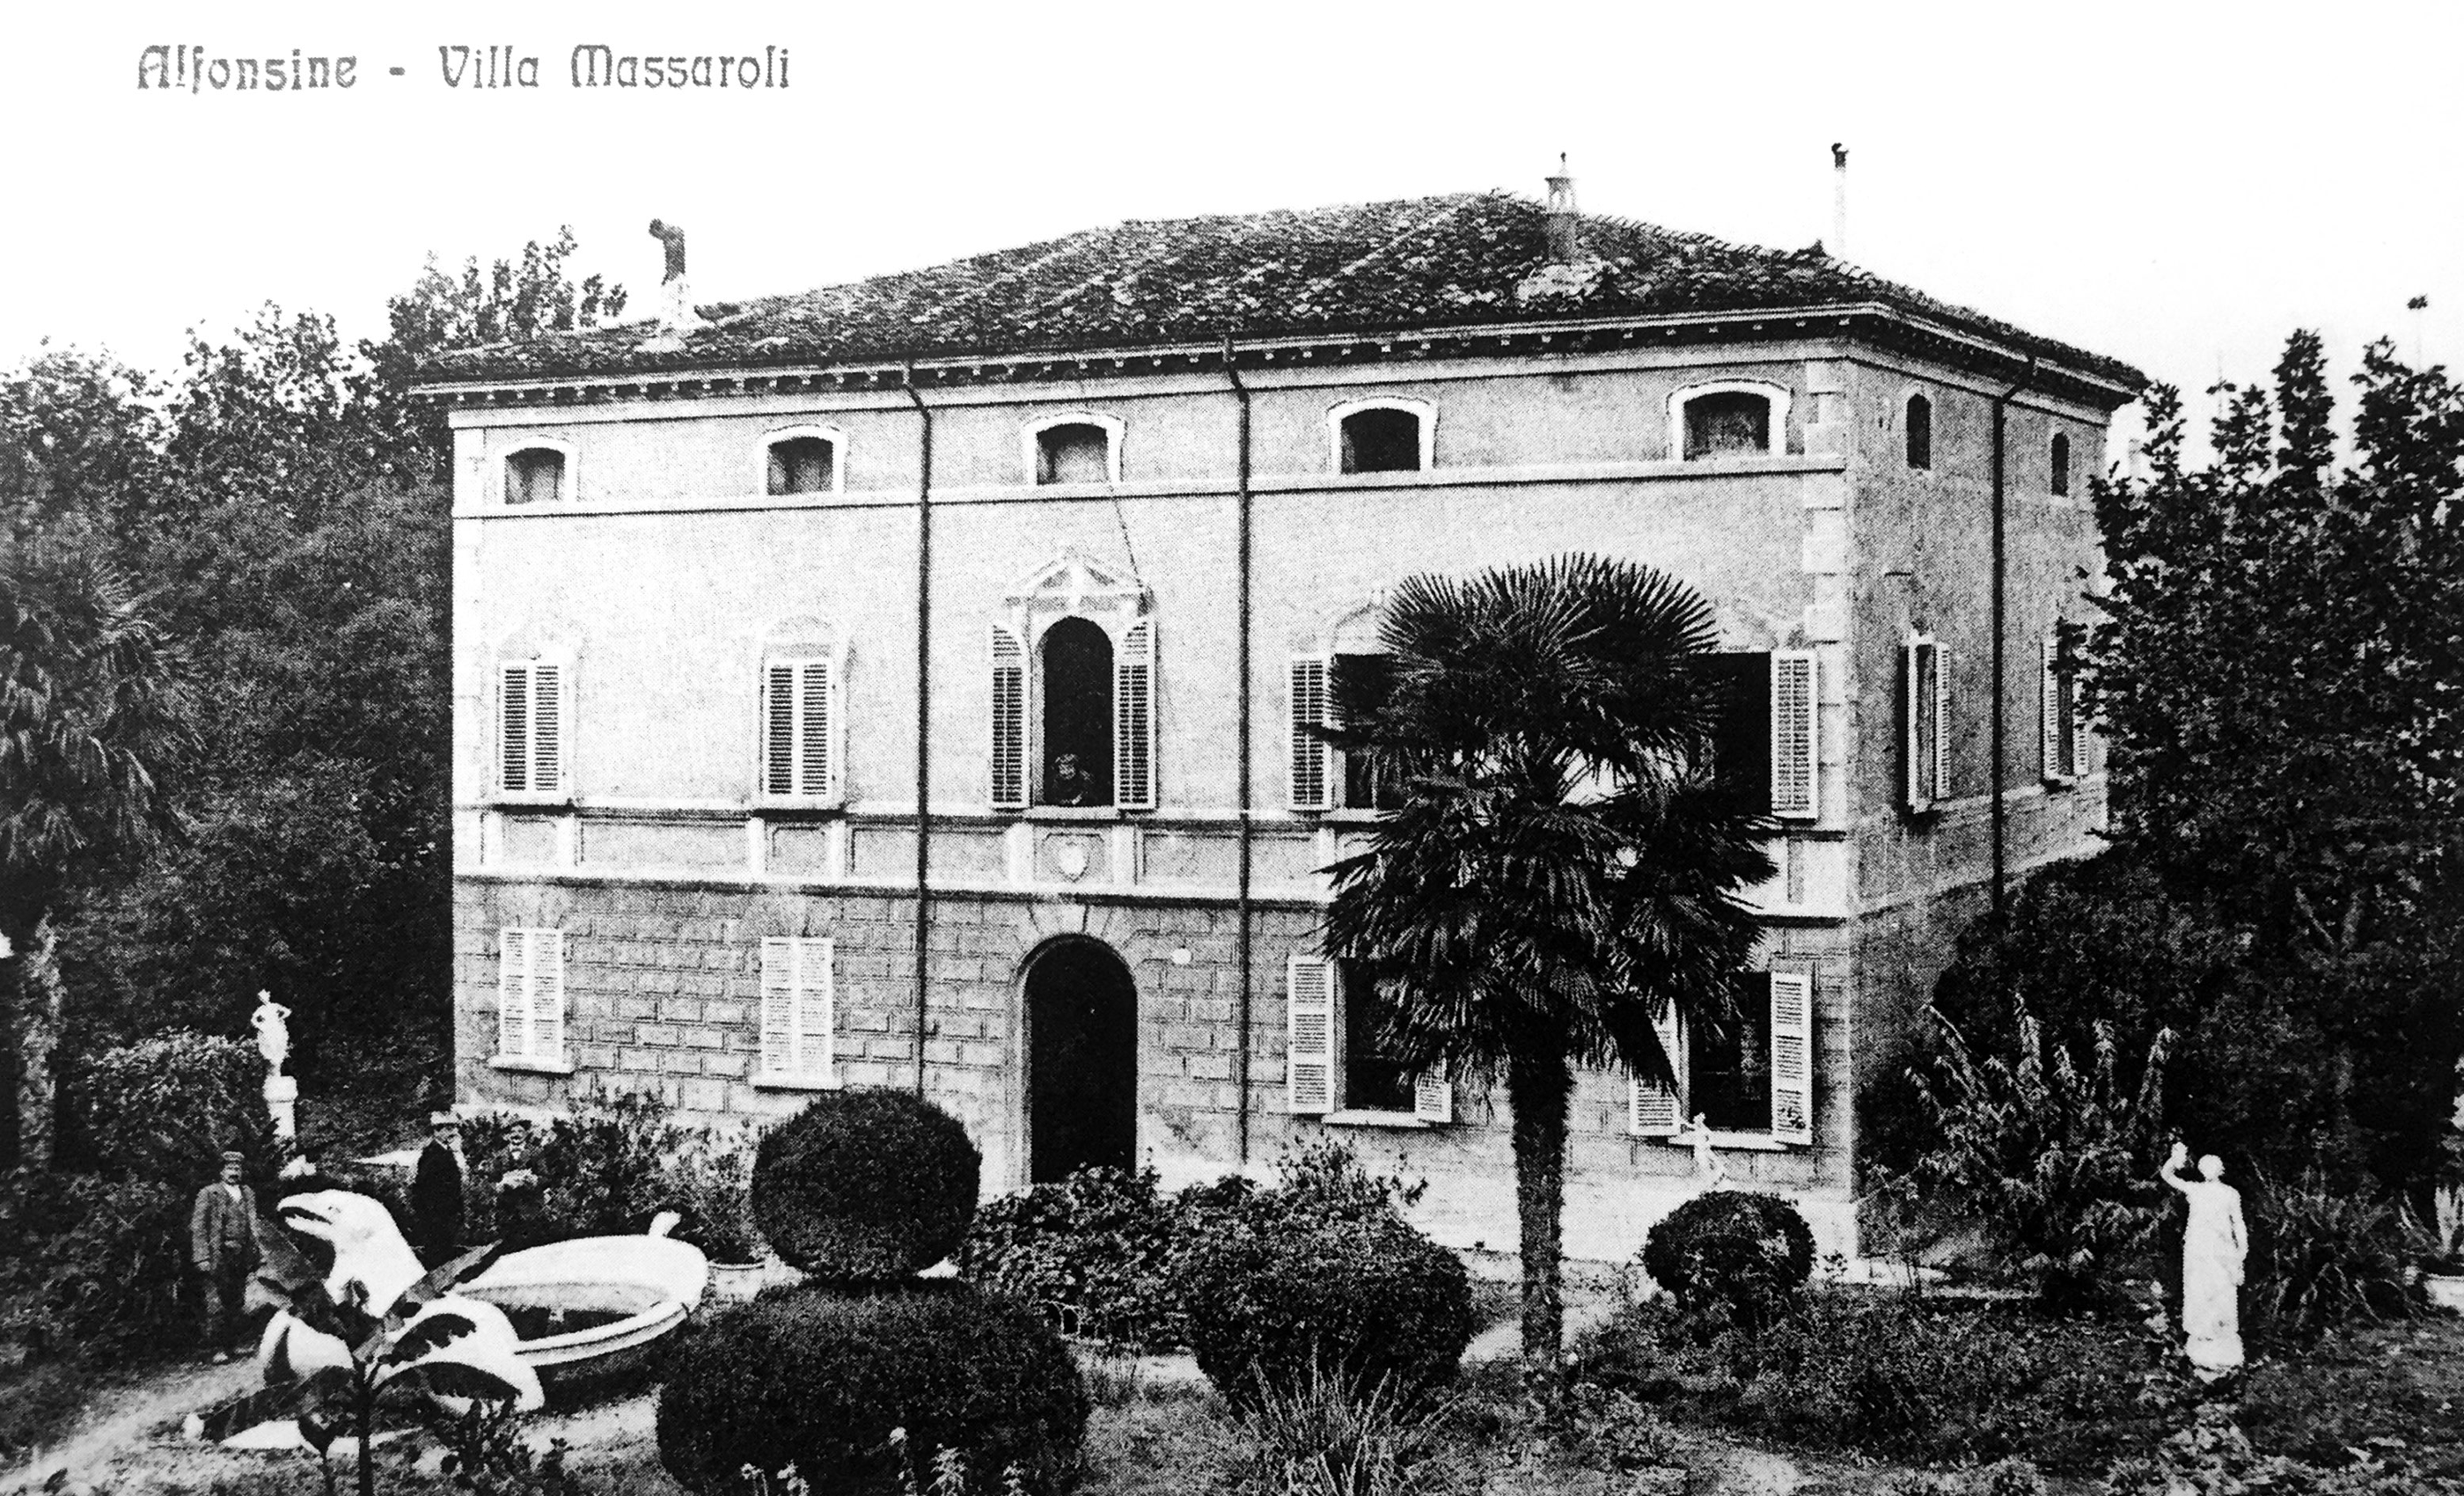
\includegraphics[width=\textwidth]{villamassaroli}
    \caption[Villa Massaroli (1940)]{
    	\index[Luoghi]{Massaroli (villa)}La \textbf{Villa Massaroli}. Era detta la `ca d'la marchesa' poiché era di proprietà della marchesa Giuditta Passari Massaroli da Recanati\index[Personaggi]{Passari Santacroce Venturi Gallerani Giuditta (marchesa)}. Sposò Giuseppe Massaroli\index[Personaggi]{Massaroli Giuseppe}, parente di Paolo Massaroli\index[Personaggi]{Massaroli Paolo}, che possedeva il palazzo che diventò Palazzo Fernè. In gergo popolare, la villa era detta `dl'ucarò', per la presenza nel giardino di fronte alla villa di una vasca con fontana a forma di un grande uccello, forse un’aquila. Non sono riuscito a capire la parentela che lega questi Massaroli, ma probabilmente sono tutti parenti poiché discendono da una famiglia che arrivò ad Alfonsine nel 1830. 
    \label{fig:villamassaroli}
    }
    %\vspace{-0.3cm}
\end{figure}